% Embedded Systems Project Report

\documentclass[12pt, english]{scrartcl}
\usepackage[a4paper,bindingoffset=0.2in,left=.5in,right=.5in,top=1in,bottom=1in,footskip=.5in]{geometry}
\usepackage[english]{babel}
\usepackage{graphicx}
\usepackage{lipsum}
\usepackage[bitstream-charter]{mathdesign}
\usepackage[T1]{fontenc}
\graphicspath{{./figures/raster/}{./figures/vector/}}

\usepackage{tabularx}
\usepackage{array}
\newcolumntype{L}[1]{>{\raggedright\let\newline\\\arraybackslash\hspace{0pt}}m{#1}}
\newcolumntype{C}[1]{>{\centering\let\newline\\\arraybackslash\hspace{0pt}}m{#1}}
\newcolumntype{R}[1]{>{\raggedleft\let\newline\\\arraybackslash\hspace{0pt}}m{#1}}
\newcolumntype{P}[1]{>{\raggedleft\arraybackslash}p{#1}}

\usepackage{textcomp}
\usepackage{xcolor}
\usepackage{mathtools}
\usepackage{numprint}
\usepackage{amsmath}
\usepackage[linesnumbered]{algorithm2e}
\usepackage{multirow}
\usepackage{multicol}
\usepackage{subcaption}
\usepackage{float}
\usepackage{url}
\usepackage{enumerate}
\usepackage{gensymb}


\usepackage{prettyref}
\newrefformat{fig}{Figure~\ref{#1}}
\newrefformat{tab}{Table~\ref{#1}}
\newrefformat{sec}{Section~\ref{#1}}
\newrefformat{ssec}{Paragraph~\ref{#1}}
\newrefformat{eq}{Equation~\ref{#1}}
\newrefformat{alg}{Algorithm~\ref{#1}}

\makeatletter
\newcommand{\redub}{}
\def\redub#1{%
  \@ifnextchar_%
    {\@redub{#1}}
    {\@latex@warning{Missing argument for \string\redub}\@redub{#1}_{}}%
}
\def\@redub#1_#2{%
    \colorlet{currentcolor}{.}%
    \color{black}%
    \underbrace{\color{currentcolor}#1}_{\color{black}#2}%
    \color{currentcolor}%
}
\makeatother

%----------------------------------------------------------------------------------------
%	My Info
%----------------------------------------------------------------------------------------
\newcommand{\horrule}[1]{\rule{\linewidth}{#1}}
\title{\normalfont \normalsize 
\textsc{Politecnico di Milano - Department of Electronics, Information and Bioengineering} \\[1cm]
\includegraphics[scale=1.2]{polimi} \\[1cm]
\horrule{0.5pt} \\[0.4cm]
\huge \textbf Porting Of Miosix OS Into An Electronic Speed Control Board For Permanent Magnet Alternating Current Motors \\[.5cm] % The assignment title
\large Coding Project \\
\horrule{2pt} \\[0.5cm]
\vfill
\author{}
\begin{tabular}{r l}
\textbf{Student} & Arturo Montufar Arreola \\
\textbf{ID} & 840541 \\[0.5cm]
\textbf{Course} & Embedded Systems \\
\textbf{Academic Year} & 2016-2017 \\[0.5cm]
\textbf{Advisor} & Federico Terraneo \\ %e.g. Simone Libutti, Giuseppe Massari
\textbf{Professor} & William Fornaciari \\
\end{tabular}
\date{\normalsize\today}
}



\begin{document} % Anything between \begin{} and \end{} is called "environment"

	\maketitle % Print the title

	\pagebreak\tableofcontents\pagebreak

	% 1 Introduction
%	(Introduction content)
%	1.1 Problem Statement:
%		- Need of electric motors
%		- Explanation of the physics
%		- Torque problem
%		- Solutions to the torque problem
%		- Introduction of the PMAC motors
%		- Explanation of PMAC motors
%		- 
%	1.2 Summary of the work
%		-
%
% 2 Design and implementation
%	2.1 VESC Board
%	2.2 Miosix Porting
%	2.3 BLDC Driving Algorithm
%	2.4 PID Controller
%
% 3 Experimental evaluation
%	3.1 Experimental Setup
%	3.2 Results
%
% 4 Conclusions and Future Works


\section{Introduction}
The development of electric motor drives is one of the topics that draws the interest of many engineers and scientists due to the multidisciplinary approach needed to reach the speed, torque and efficiency required to drive the development that the inventions of tomorrow require. The electronic approach to improve the motor driving is directly related to the development of complex control algorithms in embedded software that improve the performance of the motor. The solution proposed in this project consists in the porting of Miosix, an Operating System for embedded devices, into an Electronic Speed Control (ESC) board designed to control Permanent Magnet Alternating Current (PMAC) motors. The main intention of the project is to improve the development of the projects related to this board for future applications, creating and setting up a new board in the Miosix Kernel with a different hardware configuration, modifying the source code as least as possible and creating new modules to successfully implement a Six-Step control algorithm for a Brushless DC motor, which is one of the most efficient and accurate motor technologies available for applications which require high speed and high torque, but also it also requires a control method that is more complex than the ones used in other types of motors.
% This part is done ----------------------------------------------------------------

\subsection{Problem statement}
Nowadays, electric motors are required in a large number and variety of industrial and domestic applications, from home appliances and hand-held gadgets, to robotics and the aerospace industry. As the complexity of the application increases, also the need for accuracy and efficiency does, leading to the development of more advanced electric motor technologies and therefore, more complex motion control techniques.\\

To understand the problem being faced when driving a motor, it's necessary to briefly explain the basics of the electric motor. An electric motor is a device that transforms electric energy into mechanical energy by circulating an electric current in a rigid loop (i.e. an energized copper wire winding) which interacts with a magnetic field setup for this purpose. The principle behind this is mainly explained by the Lorentz equation for the magnetic force \cite{MaxwellEqs}

\begin{equation}
\overrightarrow{F_{B}}=q\overrightarrow{v}\times\overrightarrow{B}
\end{equation}

which states that the magnetic force $\overrightarrow{F_{B}}$ applied over a charged particle (an electron flowing in a conductive material, like a copper wire winding) is equal to the charge of the particle $q$ multiplied by its velocity $\overrightarrow{v}$ and the magnetic field $\overrightarrow{B}$ acting on it in a perpendicular direction respect to its velocity (cross product). The rigid loop used to explain this principle is a rectangular shaped loop, able to spin in one of the axes of the plane where it's placed. In \prettyref{fig:Lorentz_diagrams} we can see that a current $I$ flows though the loop in two situations: in \prettyref{fig:LorentzDiagram_a}, a magnetic field is orthogonal to the vector $\overrightarrow{S}$, which is normal to the plane of the loop; in \prettyref{fig:LorentzDiagram_b}, the magnetic field is parallel to the vector $\overrightarrow{S}$. \\

Following equation 1, we obtain a force that is applied to the sides of the loop where the circulating current direction is perpendicular to the magnetic field, therefore, there is a torque $T$ applied in the axis where the loop can spin, defined by the force $\overrightarrow{F}$ and the radius $r$. In \prettyref{fig:LorentzDiagram_a} we can easily recognize the torque by considering 2 forces "pulling" horizontally the opposite sides of the loop into opposite directions. The opposite directions of the forces applied are defined by the interaction of the circulating current with the magnetic field: when the current enters the loop, it goes in one direction, but when if comes out of the loop, the direction of the current respect to the magnetic field is the opposite. After reaching the maximum angle by pulling these sides of the loop, we reach the position shown on \prettyref{fig:LorentzDiagram_b} where there is no torque due to the overlap of the generated force vectors. \\


\begin{figure}[H]

\begin{subfigure}{.5\textwidth}
\centering\includegraphics[width=.4\linewidth]{LorentzDiagram_a} 
\caption{$\overrightarrow{S}$ perpendicular to $\overrightarrow{B}$}
\label{fig:LorentzDiagram_a}
\end{subfigure}
\begin{subfigure}{.5\textwidth}
\centering\includegraphics[width=.4\linewidth]{LorentzDiagram_b}
\caption{$\overrightarrow{S}$ parallel to $\overrightarrow{B}$}
\label{fig:LorentzDiagram_b}
\end{subfigure}
 
\caption{Torque on a conducting wire loop inside a magnetic field.}
\label{fig:Lorentz_diagrams}
\end{figure}

There are different solutions to overcome this situation where the coil doesn't move because there is no torque and to create a continuous motion with a continuous torque. For instance, the Direct Current (DC) motor uses multiple independent current loops which are energized by using brushes and mechanical commutators, changing the direction of the current in each loop after moving the rotor a few degrees, so that there is always current only in the loop which generates a useful magnetic force $\overrightarrow{F_{B}}$. Another solution to this problem is the one adopted by the Stepper motors and the PMAC motors, which instead of rotating the energized coils under a static magnetic field, energize a static coil with an electronically controlled alternating current to create a rotating magnetic force which interacts with the magnetic field attached or generated on the rotor of this type of motors.\\

The Permanent Magnet Alternating Current (PMAC) motors are preferred over the DC motors in some high speed applications because they have a better efficiency, a longer life, generate less noise, they don't require maintenance and they don't generate the sparks that the DC motors generate due to the brushes and the mechanical commutation, which might be dangerous in some environments. \\

Since the energizing of the coils of the PMAC motor depends on the angular position of its rotor to generate the best torque vs rotor-position interaction, it is necessary to electronically sample the rotor position multiple times in one single rotation to define the best driving condition to be applied on each instant. Due to this requirements, the driving methods for the PMAC motors are not trivial, so specialized embedded systems must be developed to deal with the data acquisition and motor driving in an effective, versatile and robust way. The embedded systems that deal with this kind of motors are called Electronic Speed Controllers (ESC), and its main purpose is to vary the electric motor's speed and direction.\\

To deal with the information mentioned previously, the microcontroller selected for the application must be chosen carefully, considering the speed of the motor, the accuracy and efficiency needed for the system and the external functionalities needed depending on the application. Together with the selection of the device, the software of the embedded system must be developed to reach the desired performance, which leads to the development of more complex algorithms and operating systems to run inside the embedded system.\\

\subsection{Summary of the work}
This project consisted in the porting of Miosix OS into an electronic speed control board and the development of a firmware module to control the motor driver and finally to implement the Six-Step drive algorithm to move a Brush-Less DC (BLDC) motor, which is part of the family of the PMAC motors.\\

To manage the porting of Miosix, it was required to modify some of the configuration files and the make files in the C++ project environment and to add some files that manage the configuration of the board which is using an STM32F405 microcontroller, device that was not configured previously in the Kernel. After this, another C++ class was created to manage the generation of the PWM signals according to the motor Hall effect sensors and other software inputs. Finally, to make use of the OS ported into the board, a PID control algorithm was implemented into a thread and another thread was created to manage the communication via UART with a PC using a LabView interface developed to test the system.
\pagebreak

\section{Design and implementation}
\subsection{VESC Board}

The systems employed to control the motion of electric motors are called electric drives. The electric drive can be defined as an electromechanical device that deals with the conversion of electrical energy into mechanical energy to impart motion to different machines and mechanisms for various kinds of process control \cite{GhioniElecDrives}. In the case of the PMAC motors, the electric drive consists mainly in a three-phase inverter that generates an alternating current which depends on the wanted speed of rotation and the actual angular position of the rotor. \\

\begin{figure} [H]
\centering\includegraphics[width=12cm]{ElectricDrive}
\caption{Main components of an electric drive.}
\label{fig:Electric_Drive}
\end{figure}


ESC circuits consist mainly in the following components: a processing unit, normally a microcontroller, which will control the system according to the reference value wanted and the conditions of the motor which are sensed by the same; the driver circuit, which consists in an interface between the microcontroller and the power transistors that energize the coils; the power transistors, which are selected according to the power requirements of the application; and the data acquisition module, which consists mainly in rotor angular position detection or the Hall effect signal conditioning and the current sensors that are used to avoid over-current problems or to obtain feedback for control algorithms related with current and torque control.\\

The electric drive on which this project was developed is based on an open source project developed by the Sweedish engineer Benjamin Vedder called VESC - Open Source ESC, which consists in the hardware design of a Printed Circuit Board (PCB) and the soure code used to drive a BLDC motor. The PCB was designed to be used in electric skateboards, therefore it has a small form-factor and it can be used for different applications with similar power demand. The hardware can also be modified by changing specific components to drive motors with higher power demand \cite{VedderSite}.\\

The central component in this board around which the rest of the circuit was designed is the Texas Instruments IC Brushless Motor Driver DRV8302, which is an N-type MOSFET half-bridge gate driver for three-phase motors \cite{TIDRV8302}. This device deals with the problems that high-side MOSFET switching drivers have to solve, like charge and discharge times, allowing a driving frequency up to 200 kHz, and driving the high-side gate, allowing a 100\% duty cycle. The IC also deals with safety issues, for example, it automatically avoids driving the 2 transistors in the same branch, which would create a short circuit in the board and it also detects high temperatures. Another useful feature of the IC is that it provides a step-down voltage regulator, which is used to power the other devices in the board, reducing the number of large components on the board, improving the form-factor of the device.\\

\begin{figure} [H]
\centering\includegraphics[width=14cm]{DRV8302}
\caption{DRV8302 Simplified Application Schematic}
\label{fig:DRV8302_simpSch}
\end{figure}

The selection of the transistors should be made considering the power requirements of the application. For this design, Vedder selected the Power MOSFET IRFS7530, a transistor from International Rectifier that handles up to 240 A if the temperature of the device stays under 100 \degree C \cite{TIDRV8302}. Since the motor used in the test of this project doesn't draw more than 5.4 A \cite{BLDCMotorManual}, the board was assembled with the same device.\\

The processor for which this board was designed is the STM32F405rg: a 64-pin IC microcontroller of the STMicroelectronics family of 32-bit devices with an ARM Cortex-M4 CPU and a core operating frequency up to 168 MHz. The Cortex-M4 core features a Floating point unit (FPU) single precision which supports all ARM single-precision data-processing instructions and data types. It also implements a full set of DSP instructions, which makes it ideal for the signal processing required to drive PMAC motors. This microcontroller also includes three 12-bit ADCs and supports USART, I$^2$C, SPI, USB and CAN communication interfaces, improving the versatility of the VESC board. The memory of the microcontroller consists in 1024 kB of Flash memory and 192 kB of SRAM memory \cite{STM32F405Datasheet}.

\subsection{BLDC Motor Drive Algorithm}

PMAC motors consist mainly on 3 components as shown in \prettyref{fig:PMAC_assembly}: the rotor, which has permanent magnets attached to it; the stator, which has the current carrying coils winded to it; and the end bells, which attach the rotor and the stator using bearings. As mentioned before, the motion of the PMAC motor is generated by the magnetic force generated by the interaction between the static magnetic field of the permanent magnets attached to the rotor and the alternating current flowing through the coils winded around the stator. The different configurations of the coils winding in the stator define two types of motors: the BLDC motor, which has trapezoidal Back Electro-Motive Force (BEMF) and the Permanent Magnet Synchronous Motor (PMSM), which has sinusoidal BEMF. The Back Electro-Motive Force is the voltage generated in the coils due to the rotation of the magnetic field inside the windings loop, which creates a current that opposes to the movement of the magnetic field, as stated by Lenz Law \cite{MaxwellEqs}. The current that flows through the windings to drive the motor should be shaped accordingly to the shape of its BEMF to obtain the maximum efficiency possible, which is one of the reasons why the BLDC motor is widely used, since its driving signal is easier to implement due to the trapezoidal shape of its BEMF which can be generated by just alternating polarities in a three-phase inverter, while the PMSM needs a more complex algorithm to generate a three-phase sinusoidal signal. In some applications it's preferred to use PMSM because they can reach an efficiency up to 94\% and their drive generates lower harmonic components than the BLDC drive \cite{GuoPMSMefficiency2016}.\\ 

\begin{figure} [H]
\centering\includegraphics[width=10cm]{bldcAssembly}
\caption{Assembly details of a typical PMAC motor.}
\label{fig:PMAC_assembly}
\end{figure}

As mentioned before, the control of the current direction in the PMAC motors must be done electronically instead of mechanically like in the DC motors. In the case of the BLDC motors, the stator windings must be energized in a sequence depending on the rotor position. There are different methods to detect the rotor angular position, but the simplest one for the BLDC motor is to use Hall effect sensors, which are normally attached to the stator and close to the rotor so to detect the magnetic field of the magnets attached to it. When the rotor magnetic poles pass near the sensor, the sensor delivers a high or low signal to the microcontroller. The combination of signals delivered by the Hall effect sensors determines the sequence that has to be applied to move the motor correctly.

\begin{figure} [H]
\centering\includegraphics[width=12cm]{bldcInverter}
\caption{Three phase inverter consisting in 3 half-bridge inverters.}
\label{fig:BLDC_Inverter}
\end{figure}


\begin{figure} [H]
\centering\includegraphics[width=12cm]{DriveDiagram}
\caption{At every 60 electrical degrees of rotation of the rotor's magnetic field, there is a change in the state of the Hall effect sensors.}
%include citation to Microchip Application note
\label{fig:BLDC_pulses_sequence}
\end{figure}

\newcolumntype{C}{>{\centering\arraybackslash}p{2em}}

\begin{table}
\small
\begin{center}
\caption{Sequence for rotating the motor}
\begin{tabular}{|c|C|C|C|c|c|C|C|C|}
\hline
\multicolumn{9}{|c|}{Clockwise Direction} \\ \hline \hline
\multirow{2}{*}{Sequence \#} & \multicolumn{3}{c|}{Hall Sensor Input} & \multicolumn{2}{c|}{Active Gates} & \multicolumn{3}{c|}{Phase Current} \\ \cline{2-9} 
  & A & B & C & High Side & Low Side & A & B & C \\ \hline \hline
1 & 1 & 0 & 0 & $Q_B+$ & $Q_A-$ & DC- & DC+ & Off       \\ \hline
2 & 1 & 0 & 1 & $Q_C+$ & $Q_A-$ & DC- & Off & DC+       \\ \hline
3 & 0 & 0 & 1 & $Q_C+$ & $Q_B-$ & Off & DC- & DC+       \\ \hline
4 & 0 & 1 & 1 & $Q_A+$ & $Q_B-$ & DC+ & DC- & Off       \\ \hline
5 & 0 & 1 & 0 & $Q_A+$ & $Q_C-$ & DC+ & Off & DC-       \\ \hline
6 & 1 & 1 & 0 & $Q_B+$ & $Q_C-$ & Off & DC+ & DC-       \\ \hline \hline
\multicolumn{9}{|c|}{Counter-Clockwise Direction} \\ \hline \hline
\multirow{2}{*}{Sequence \#} & \multicolumn{3}{c|}{Hall Sensor Input} & \multicolumn{2}{c|}{Active Gates} & \multicolumn{3}{c|}{Phase Current} \\ \cline{2-9} 
  & A & B & C & High Side & Low Side & A & B & C \\ \hline \hline
1 & 1 & 0 & 0 & $Q_A+$ & $Q_B-$ & DC+ & DC- & Off       \\ \hline
2 & 1 & 0 & 1 & $Q_A+$ & $Q_C-$ & DC+ & Off & DC-       \\ \hline
3 & 0 & 0 & 1 & $Q_B+$ & $Q_C-$ & Off & DC+ & DC-       \\ \hline
4 & 0 & 1 & 1 & $Q_B+$ & $Q_A-$ & DC- & DC+ & Off       \\ \hline
5 & 0 & 1 & 0 & $Q_C+$ & $Q_A-$ & DC- & Off & DC+       \\ \hline
6 & 1 & 1 & 0 & $Q_C+$ & $Q_B-$ & Off & DC- & DC+       \\ \hline
\end{tabular}
  \label{tab:drive_sequence}
\end{center}
\end{table}


The simplest driving method for this type of motors is called Six-Step drive, and consists in energizing each winding of the three-phase system for 120 degrees and leaving the winding de-energized for 60 degrees as seen in \prettyref{fig:BLDC_pulses_sequence}. To achieve this, a three-phase inverter is used. This three-phase inverter consists in 3 half-bridges (\prettyref{fig:BLDC_Inverter}) which are driven following a six-steps commutation sequence, as indicated in \prettyref{tab:drive_sequence}, that develops the most amount of torque possible according to the rotor position detected by the Hall effect sensors. The motor is driven by energizing 2 phases at a time (current enters the first winding and exits the second winding) and leaving the third phase floating. In order to keep the motor running, the magnetic field produced by the windings should shift position, as the rotor moves to catch up with the stator field. This method is implemented in the embedded software by calling the function $trapezoidalDrive()$ in an interruption of the timer $TIM2$ at a frequency that can be determined and modified depending on the motor specifications.\\

The speed of a PMAC motor depends linearly on the voltage applied on its coils \cite{GhioniElecDrives}. In the case of the BLDC motor, since the driving is made by a six-step commutation sequence using a three-phase inverter, the voltage applied in the coils can be changed by applying a PWM signal in the gates of the transistors, this way, the voltage applied in the coils is a percentage of the main source voltage $V_{DC}$ equal to the duty cycle of the PWM applied.\\


The speed of the motor can be easily calculated by counting each time that the interruption from $TIM2$ is called and the Hall effect sensor hasn't moved from a certain position to another. This speed obtained is used later to implement the PID controller, since it needs a reference value to reach and an error signal to close the control loop.

\subsection{PID Controller}
Proportional-Integral-Derivative (PID) control is the most common control algorithm used in industry and has been universally accepted in industrial control. The popularity of PID controllers can be attributed to their robust performance in a wide range of operating conditions and to their functional simplicity, which allows engineers to operate them in a simple manner \cite{NIPID}.\\

\begin{figure} [H]
\centering\includegraphics[width=12cm]{PID}
\caption{Block diagram of a basic PID control algorithm}
\label{fig:PID_block_diagram}
\end{figure}

As seen in \prettyref{fig:PID_block_diagram}, the PID controller continuously calculates an error signal $e(t)$, which is the difference between the desired or "reference" output value and the actual measured output value. This error signal is applied to a correction factor based on proportional, integrative and derivative terms (P, I and D respectively) which automatically applies an accurate and responsive correction to the plant of the system to obtain the wanted output value. Each one of the PID terms are obtained with different calculations of the error signal. The proportional term is set proportionally to the output error, therefore it changes depending on the actual error signal and a proportional factor $K_p$. The integral term of the controller increases its value not only depending on the error value, but also depending on the amount of time that the error has persisted, therefore, if a value applied to reduce the error is not enough, the value will increase, depending on the $K_i$ value, until the error starts decreasing. The last term is the derivative, which doesn't consider the error value, but it considers its rate of change and tries to reduce it with a value that depends on the derivative factor $K_d$. The selection of the PID controller factors is called "tunning" and it depends completely on the application requirements.\\

In the case of this project, the PID controller was used to control the speed of the motor changing the duty cycle with which the transistors are driven to energize the coils of the BLDC motor depending on the speed obtained by the reading of the Hall-effect sensors.\\

The discrete version of the PID controller was implemented in this project by obtaining an error signal every time that the system is updated and following the next steps:

\begin{enumerate}
\item Store the previous error value: $err\_1 = err\_0$
\item Store the previous integral error value: $intErr\_1 = intErr\_0$
\item Obtain the new normalized error value: $err\_0 = (ref\_speed - actual\_speed) / max\_speed$
\item Calculate the new integral error value: $intErr\_0 = intErr\_1 + err\_0$
\item Calculate the derivative error value: $derErr = err\_0 - err\_1$
\item Calculate the proportional term value: $pTerm = kp * err\_0$
\item Calculate the integral term value: $iTerm = ki * intErr\_0 * dt$
\item Calculate the derivative term value: $dTerm = kd * derErr / dt$
\item Calculate the overall contribution contribution of the controller: $q = pTerm + iTerm + dTerm$
\item Update the duty cycle of the High-Side transistors according to the Six-Step drive sequence: $dutyCycle += q$
\end {enumerate}

\subsection{Miosix Porting and Implementation of BLDC Driving and Control Algorithms}
Miosix is an OS kernel designed to run on 32-bit microcontrollers, such as the one included in the VESC board. The difference between Miosix and other operating systems designed for embedded systems is that it supports C++ instead of just C, which allows the use of the multiple threads application model where applications are statically linked with the kernel. Miosix also has a multiprocess environment which allows the use of memory protection methods used in C++ \cite{MiosixSite}.\\

The process of the development to port Miosix into the VESC board can be followed in the Git repository stored in GitHub \url{https://github.com/SAHARVM/PolimiEmbedded/commits/master}, which consisted mainly in the following steps:

\begin{enumerate}
	\item Full Miosix Clone. 
		\begin {itemize}
			\item Copy of the repository containing the latest stable version of Miosix by the 21st of January into this project's repository.
		\end {itemize}
	\item First Compilation.
		\begin {itemize}
			\item Edited the lines that must be commented which force the user to modify the header file $miosix\_settings.h$.
			\item The changes to this file and the selection of a microcontroller in the $Makefile.inc$ file allow the compilation of the code.
			\item This change was made just to test the IDE configuration that must be done following the guideline available in the Miosix Wiki \url{https://miosix.org/wiki/index.php}, therefore, the code was not yet safe to be flashed into the VESC Board.
		\end {itemize}
	\item Makefile Changes
		\begin {itemize}
			\item Modified the file $Makefile.inc$ of the Miosix kernel to include the VESC Board naming it $stm32f405RGTx\_VESC\_4\_12$ since the VESC Board model used in the project is the version 4.12
			\item The changes included the creation of the path which contains the architecture files of the board and the specification of the ROM and RAM memories to 1 MB Flash and 192+4 KB RAM \cite{STM32F405Datasheet} and the Clock frequency to 168 MHz.
		\end {itemize}
	\item Porting Files Creation
		\begin {itemize}
			\item The board required the inclusion of the following files, which were copied from the architecture files of the $stm32f407vg\_bitsboard$ configuration since the microcontrollers STM32F405 and STM32F407 have almost the same characteristics:
				\begin {itemize}
					\item $stage\_1\_boot.cpp$
					\item $arch\_registers\_impl.h$
					\item $bsp.cpp$
					\item $bsp\_impl.h$
					\item $stm32\_256k+64k\_rom.ld$ later changed to $stm32\_1m+192k\_ram.ld$
					\item $stm32f405RGTx\_VESC\_4\_12.cfg$
					\item $board\_settings.h$
					\item $c\_standard\_headers\_indexer.c$
					\item $cpp\_standard\_headers\_indexer.cpp$
				\end {itemize}
			\item The main change in the configuration of the VESC board with respect to the "base" one was the memory configuration which consists in 1024 kB of Flash memory and 192 kB of SRAM as mentioned previously.
		\end {itemize}
	\item STM32CubeMX Files
		\begin {itemize}
			\item This commit consisted in the attempt to use the Hardware Abstraction Layer (HAL) library and the files generated by the software generation program STM32CubeMX by STMicroelectronics to automatically configure the peripherals of the VESC Board microcontroller. Later on, this idea was discarded since the STM32 library version that Miosix uses for this was an earlier version than the one that STM32CubeMX uses and some macros and definitions were different. There were so many changes to do that it made no sense to try it, so the configuration of the microcontroller peripherals was made by hand and the included files were deleted in the next commit.
		\end {itemize}
	\item First Working Test - LED blink
		\begin {itemize}
			\item For this commit, the idea was to configure one of the pins of the microcontroller that was connected to a LED to prove that the porting was successful.
			\item The changes to achieve this consisted mainly in the modification of the files $bsp.cpp$ and $bsp\_impl.h$.
			\item This commit also included the change in the configuration of the system to work with the serial port number three, since it's the only one accessible in the VESC Board and Miosix doesn't support the USB CDC serial communication available in the microcontroller.
		\end {itemize}
	\item GPIO Configuration
		\begin {itemize}
			\item One of the changes of this commit consisted in the configuration of the other available LED
			\item The other change consisted in the first modifications of the file $servo\_stm32.cpp$ to generate a PWM signal in a port available in the VESC Board to drive an RC servomotor, which doesn't coincide with the ports configured in the original file.
		\end {itemize}
	\item Servomotor File Modification Working
		\begin {itemize}
			\item After understanding the configuration of the timer connected to the pin that needed to be configured, $TIM3$, the PWM signal was generated in the wanted peripheral. This code was the base of the creation of the file which is used to generate the PWM signal for the driving of the BLDC motor using the advanced timer $TIM1$.
		\end {itemize}
	\item PMAC Driver Class Creation
		\begin {itemize}
			\item To achieve the goal that consisted in avoiding the modification of the original files, a new file was created to control the PWM signals corresponding to the available RC servomotor port and the 6 PWM signals needed to drive the BLDC motor.
			\item For this commit, the new file only configured the PWM signal of the servomotor output.
		\end {itemize}
	\item Hall effect Sensors Read
		\begin {itemize}
			\item Inclusion of the functions to obtain the state of the Hall effect sensors to drive the BLDC motor accordingly
		\end {itemize}
	\item Thread Implementation
		\begin {itemize}
			\item Included the use of threads to drive the test signal
		\end {itemize}
	\item Configuration of Timer 1
		\begin {itemize}
			\item The microcontrollers STM32F405xx and STM32F407xx have two PWM timers that include specific functions to generate 6 PWM signals for PMAC motor control. With this purpose, the VESC Board has the output pins of timer $TIM1$ connected to the gate drivers of the DRV8203 IC. For this commit, 3 of the 6 signals related to this timer output were configured to drive the BLDC motor.
		\end {itemize}
	\item Implementation of the Trapezoidal Drive
		\begin {itemize}
			\item For this commit, an attempt to drive the BLDC motor using a thread with a 1 ms delay was made. The motor worked correctly until the 40\% of the duty cycle but since the speed of the motor increases linearly as the duty cycle increases, the 1 kHz frequency of the thread was not fast enough for bigger speeds.
			\item Another thread was created to communicate the VESC Board with a serial monitor in a PC using a USB-Serial board attached to it. This allows the modification of some parameters of the board, like the duty cycle, and the reading of some other parameters, like the motor speed.
		\end {itemize}
	\item Trapezoidal Drive at $TIM2$ Interrupt
		\begin {itemize}
		\item Since the algorithm to drive the motor must run at around 50 kHz, which is a frequency much faster than the one achievable using threads (1 kHz), the timer $TIM2$ was configured to generate interruptions at that frequency to run the driving function of the motor, which reads the Hall effect sensors and according to this and to the input desired duty cycle generates a signal that moves the BLDC motor.
		\end {itemize}
	\item Speed PID Controller
		\begin {itemize}
		\item To implement a thread in a useful way, a simple PID controller algorithm was implemented. The input for the controller is a reference desired speed and the output is a PWM duty cycle. The implementation is explained later in the report.
		\end {itemize}
	\item LabView Control Interface
		\begin {itemize}
		\item To control the board in an automatic way and to obtain information from it, it was necessary to generate an interface. To achieve this, a communication method was implemented between the VESC Board using the serial port and a LabView program that interacts with the board though the USB-serial circuit. In this commit, the serial instructions were modified to control the board in an automatic way without the use of a serial monitor. This changes also include the modification of the wanted speed and the PID controller parameters.
		\end {itemize}
\end{enumerate}

Note: Some commits are not mentioned because there were some errors or are not important for the development of the project.\\

\pagebreak

\section{Experimental evaluation}
\subsection{Experimental setup}
The experimental configuration of the system consisted in connecting the VESC Board to 24V power source and a BLDC motor model DB42S03 manufactured by Nanotec \cite{BLDCMotorManual}. The motor has 8 poles per phase, which means that each mechanical revolution of the rotor requires to run the driving sequence of the coils 8 times. This last characteristic is important to calculate the mechanical speed of the motor using the Hall-effect sensors.\\

A new VESC board was bought and soldered with the components specified in the VESC Board files. Since Miosix doesn't support the use of CDC USB serial communications, it was necessary to attach a USB-Serial board to deal with the communication with the PC. An ST-LINK V2 in-circuit debugger and programmer was used to upload the code to the STM32F405rg microcontroller connected to the STM32 ST-LINK Utility software.\\

As mentioned before, to run the tests automatically, a visual interface was developed using LabView, a software platform developed by National Instruments used to create scripts in "blocks" code. The script developed for this tests consists in the use of communication blocks to send requests to the VESC board and to plot the information returned by it. For example, to set up a speed that must be achieved by the motor using the PID algorithm programmed in the VESC, the script sends a request to the board to reach a certain speed (in degrees per second) and every 100 milliseconds the script asks the board for the motor's current speed and plots it. It is also possible to implement a periodic "step" signal, which is widely used in control testing to review the behaviour of the devices and consists in abruptly changing the desired speed of the motor to see the response of the controller algorithm.\\

\begin{figure} [H]
\centering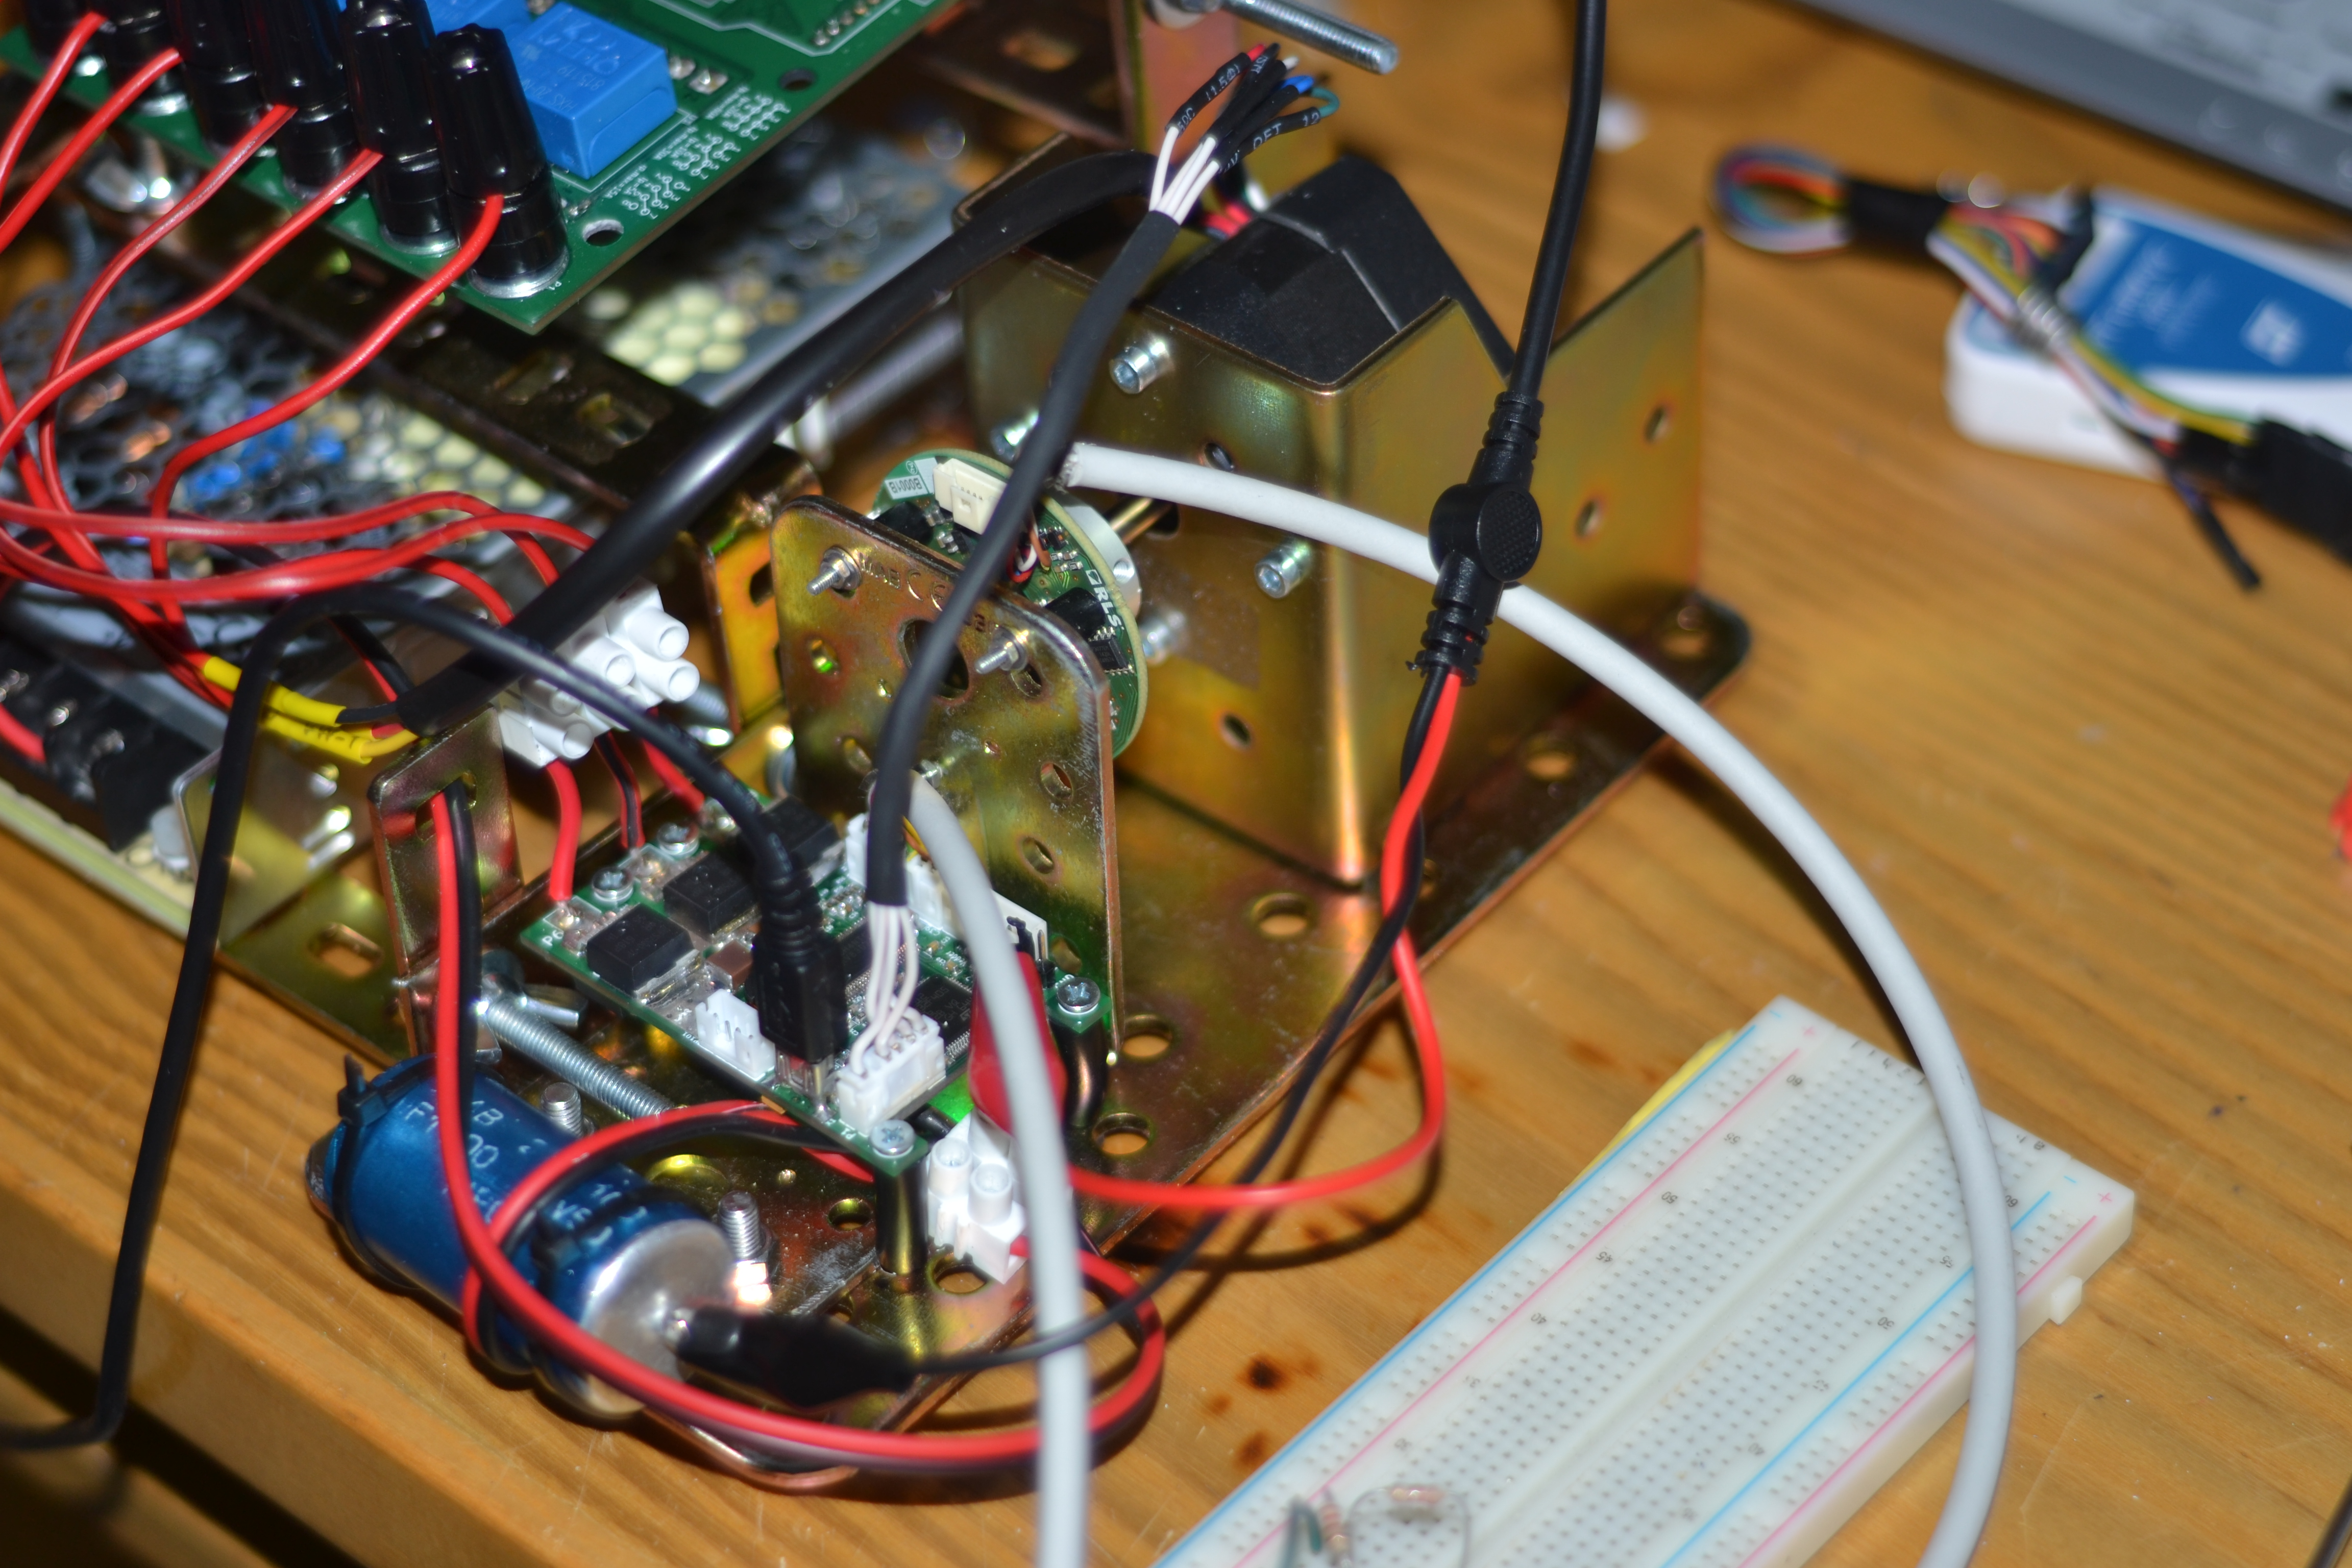
\includegraphics[width=15cm]{vesc_1}
\caption{Picture of the experimental setup}
\label{fig:VESC_1}
\end{figure}

\begin{figure} [H]
\centering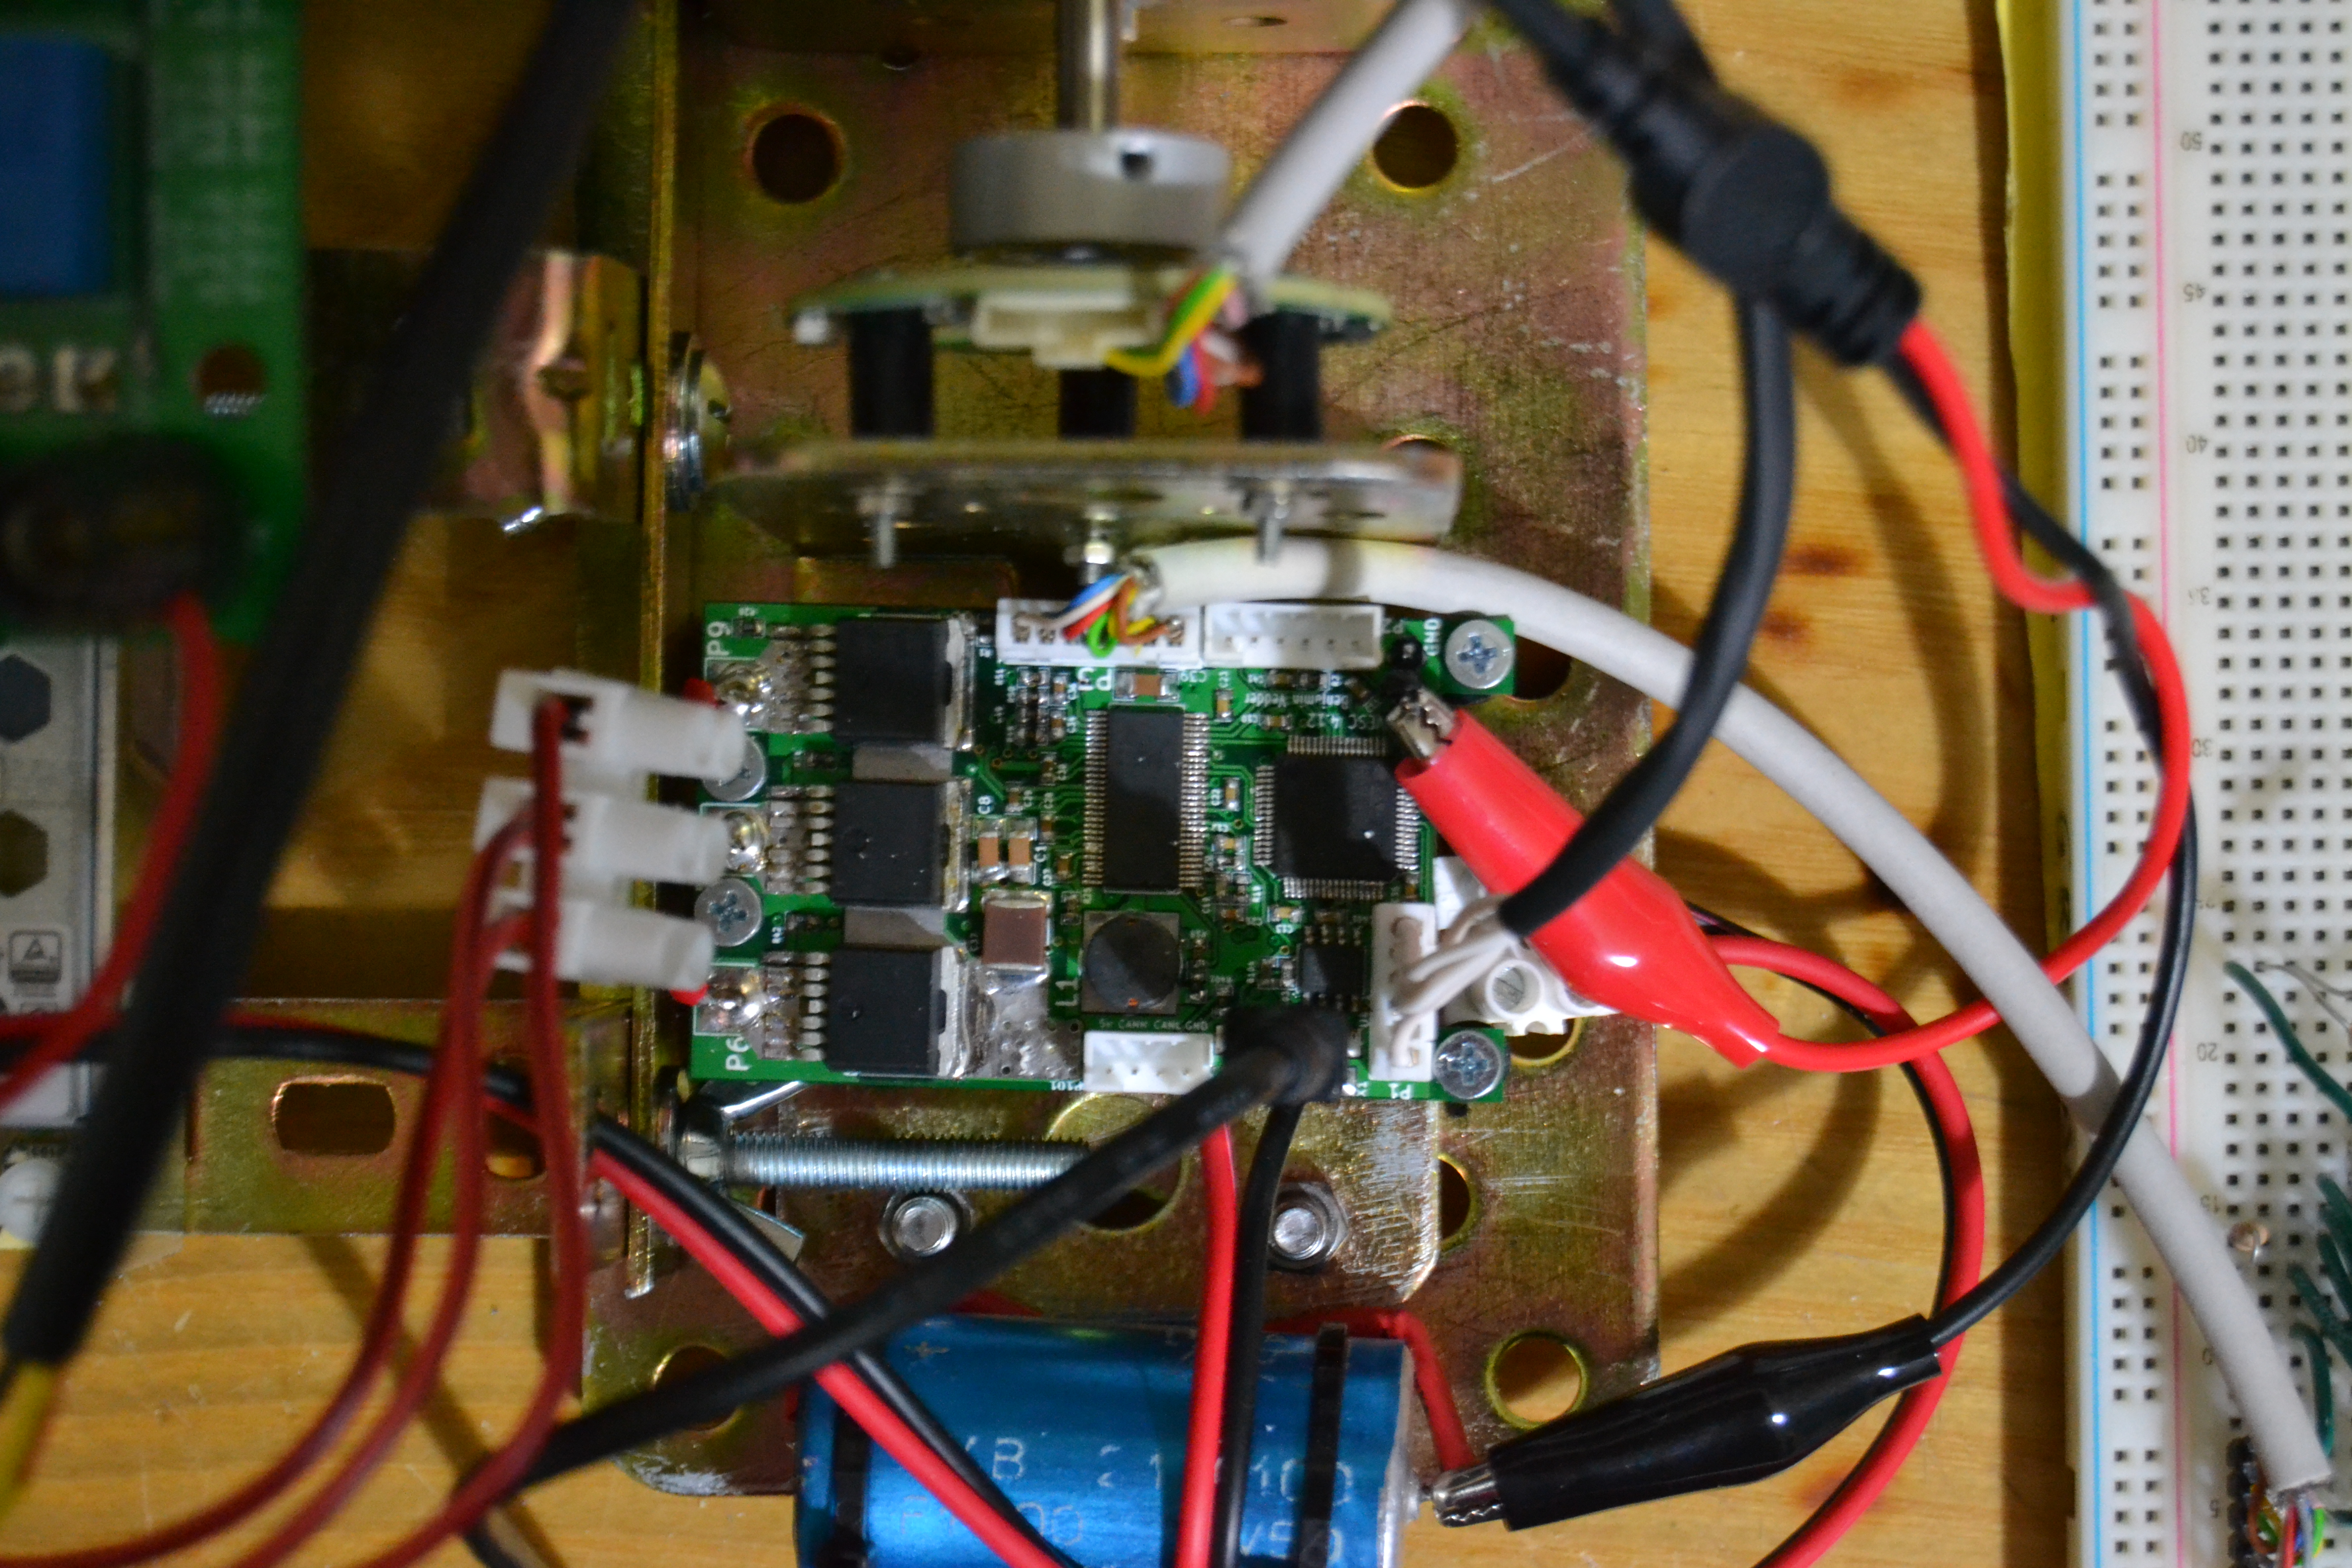
\includegraphics[width=15cm]{vesc_2}
\caption{Picture of the VESC Board connected to the external peripherals}
\label{fig:VESC_2}
\end{figure}

\begin{figure} [H]
\centering\includegraphics[width=17cm]{LabView}
\caption{Screen shot of the visual interface implemented in LabView}
\label{fig:LabView}
\end{figure}

\subsection{Results}

After porting Miosix into the VESC board, the first result was to see one of the available LEDs blinking, which was the first evidence that Miosix was successfully flashed into the microcontroller.\\

All the test results related to the motor driving are documented as oscilloscope readings or LabView plots. In the next three images (\prettyref{fig:dutycycle_10}, \prettyref{fig:dutycycle_50} and \prettyref{fig:dutycycle_100}) it is possible to see the different phase-voltage waveforms generated after applying the six-step drive algorithm at a frequency of 50kHz to drive the three-phase inverter gates at a frequency of 25 kHz. The generation of these waveforms means that the BLDC motor is successfully rotating due to the electronic commutation of the three-phase inverter, otherwise, the BEMF, seen in the images as the ramp before and after the pulses, wouldn't be seen.

\begin{figure} [H]
\centering\includegraphics[width=14cm]{10_dc}
\caption{Voltage Signal obtained applying a 10\% duty cycle}
\label{fig:dutycycle_10}
\end{figure}

\begin{figure} [H]
\centering\includegraphics[width=14cm]{50_dc}
\caption{Voltage Signal obtained applying a 50\% duty cycle}
\label{fig:dutycycle_50}
\end{figure}

\begin{figure} [H]
\centering\includegraphics[width=14cm]{100_dc}
\caption{Voltage Signal obtained applying a 100\% duty cycle}
\label{fig:dutycycle_100}
\end{figure}

Since the six-step driving algorithm can be implemented without the need of an operating system, there was no sense in having ported Miosix without using threads, therefore, the previously mentioned PID controller was implemented using a thread and also another thread was created to control the serial communication with the LabView interface, which would have been complicated to implement without an operating system. Since Miosix supports the standard C++ libraries, it also includes the console input and output commands using a serial port as a if it was PC console. This was used to implement the previously mentioned interface in just a few hours.\\

The following images were obtained using the developed LabView interface and they demonstrate the response of the BLDC motor using the PID controller implemented in a thread that is called every millisecond. As it can be seen, by changing the parameters $K_P$ and $K_I$, the behaviour of the motor changes, going from underdamped with low $K_P$ values as seen in figures \prettyref{fig:PID_2}, \prettyref{fig:PID_1} and \prettyref{fig:PID_9}, to a rough underdamping seen in \prettyref{fig:PID_3}, critically damped in \prettyref{fig:PID_5} and overdamped in \prettyref{fig:PID_7}. It can also be seen that if the parameters are not set up correctly, unstable behaviours can be obtained as seen in \prettyref{fig:PID_6} and \prettyref{fig:PID_8}. It can also be noticed that the derivative term is not used. Normally in motor control applications, the control method is only proportional and integral (PI) because since the motor dynamics are much slower than the electric dynamics and the derivative action is sensitive to small changes like noise, this might lead to destabilize the system or to take longer to reach a steady state.

\begin{figure} [H]
\centering\includegraphics[width=12cm]{PID_2}
\caption{Speed of the motor applying a step speed request with $K_P$ = 0.01, $K_I$ = 0.05 and $K_D$ = 0}
\label{fig:PID_2}
\end{figure}

\begin{figure} [H]
\centering\includegraphics[width=12cm]{PID_1}
\caption{Speed of the motor applying a step speed request with $K_P$ = 0.005, $K_I$ = 0.05 and $K_D$ = 0}
\label{fig:PID_1}
\end{figure}

\begin{figure} [H]
\centering\includegraphics[width=12cm]{PID_9}
\caption{Speed of the motor applying a step speed request with $K_P$ = 0.004, $K_I$ = 0.05 and $K_D$ = 0}
\label{fig:PID_9}
\end{figure}

\begin{figure} [H]
\centering\includegraphics[width=12cm]{PID_3}
\caption{Speed of the motor applying a step speed request with $K_P$ = 0.05, $K_I$ = 0.05 and $K_D$ = 0}
\label{fig:PID_3}
\end{figure}

%\begin{figure} [H]
%\centering\includegraphics[width=12cm]{PID_4}
%\caption{Speed of the motor applying a step speed request with $K_P$ = 0.005, $K_I$ = 0.01 and $K_D$ = 0}
%\label{fig:PID_4}
%\end{figure}

\begin{figure} [H]
\centering\includegraphics[width=12cm]{PID_5}
\caption{Speed of the motor applying a step speed request with $K_P$ = 0.005, $K_I$ = 0.001 and $K_D$ = 0}
\label{fig:PID_5}
\end{figure}

\begin{figure} [H]
\centering\includegraphics[width=12cm]{PID_7}
\caption{Speed of the motor applying a step speed request with $K_P$ = 0.001, $K_I$ = 0.001 and $K_D$ = 0}
\label{fig:PID_7}
\end{figure}

\begin{figure} [H]
\centering\includegraphics[width=12cm]{PID_6}
\caption{Speed of the motor applying a step speed request with $K_P$ = 0.001, $K_I$ = 0.01 and $K_D$ = 0}
\label{fig:PID_6}
\end{figure}

\begin{figure} [H]
\centering\includegraphics[width=12cm]{PID_8}
\caption{Speed of the motor applying a step speed request with $K_P$ = 0.001, $K_I$ = 0.05 and $K_D$ = 0}
\label{fig:PID_8}
\end{figure}


\pagebreak

\section{Conclusions and Future Works}
This project covered the development of the implementation of a six-step driving algorithm and the application of a PID controller in a BLDC motor using Miosix. Since the driving of the motor was successful allowing in a parallel way the communication with a LabView interface and the application of the PID controller which requires floating point calculations, it can be concluded that the porting of Miosix will be a useful tool for the development of future applications with the VESC board.\\

For future developments, it is planned to implement other driving algorithms using the VESC board. One of this algorithms is called Field-Oriented Control (FOC) and it requires to read and analyse the current of the motor at a given frequency to generate a sinusoidal output that must be calculated at each instant of time available. To do this calculations in parallel with CAN communication and other types of signal monitoring (like temperature) it will be very useful to have the option of implementing threads this C++ environment that Miosix offers.\\
\pagebreak

\section{Appendix}

\subsection{Appendix A: VESC Board Schematic}

\begin{figure} [H]
\centering\includegraphics[width=22cm, angle = 90]{VESC_SCH}
%\caption{Block Schematic of the VESC Board}
\label{fig:VESC_SCH}
\end{figure}

\pagebreak

\subsection{Appendix B: DB42S03 Datasheet}
\begin{figure} [H]
\centering\includegraphics[width=22cm, angle = 90]{motorDS}
%\caption{Block Schematic of the VESC Board}
\label{fig:motorDS}
\end{figure}
\pagebreak

\subsection{Appendix C: LabView VI}
\begin{figure} [H]
\centering\includegraphics[width=12cm]{VI_1}
%\caption{Block Schematic of the VESC Board}
\label{fig:VI_1}
\end{figure}

\begin{figure} [H]
\centering\includegraphics[width=12cm]{VI_2}
%\caption{Block Schematic of the VESC Board}
\label{fig:VI_2}
\end{figure}

\begin{figure} [H]
\centering\includegraphics[width=12cm]{VI_3}
%\caption{Block Schematic of the VESC Board}
\label{fig:VI_3}
\end{figure}

\begin{figure} [H]
\centering\includegraphics[width=12cm]{VI_4}
%\caption{Block Schematic of the VESC Board}
\label{fig:VI_4}
\end{figure}
\pagebreak

	\pagebreak

	\bibliographystyle{unsrt}
	\bibliography{text/project_bibliography}

\end{document}